\documentclass{scrreprt}
\usepackage{graphicx}
\usepackage{listings}
\usepackage{underscore}
\usepackage[bookmarks=true]{hyperref}
\hypersetup{
    bookmarks=false,    % show bookmarks bar?
    pdftitle={Software Requirement Specification},    % title
    pdfauthor={Yiannis Lazarides},                     % author
    pdfsubject={TeX and LaTeX},                        % subject of the document
    pdfkeywords={TeX, LaTeX, graphics, images}, % list of keywords
    colorlinks=true,       % false: boxed links; true: colored links
    linkcolor=blue,       % color of internal links
    citecolor=black,       % color of links to bibliography
    filecolor=black,        % color of file links
    urlcolor=purple,        % color of external links
    linktoc=page            % only page is linked
}%
\def\myversion{1.0}
\date{}
\usepackage{hyperref}
\begin{document}
\begin{titlepage}
  \flushright\bfseries\huge
  \vspace*{\stretch{0.4}}
    \rule{\linewidth}{5pt}
    \par
    \vspace{1cm}
    {\Huge DESIGN \par DOCUMENT \par}
    \vspace{2cm}
    for \\
    \vspace{2cm}
    Personal Dietary Application \\
    \vspace{2cm}
     \LARGE{Version \myversion \\}
    \vspace{2cm}
    by Craig Boucher \\
    Tanveer \\
    Fan \\
    Osman \\
    Xin
    \vspace{2cm}
    \rule{\linewidth}{5pt}
    \vspace{\stretch{1}}
\end{titlepage}
\tableofcontents
\chapter{Introduction}
The project undertaken in this COMP 5541 course involves creating an application that keeps track of dietary records for the user. This diet app has been designed to use the border pane layout for the main window. \\ \\ 
This design document will provide details for the type of software architecture used to develop the software and explain the design for the user interface. The architectural component illustrates the abstraction of the software classes involved and how they relate to each other to maniuplate and process data that the user interacts with. The interface design section will assess the process for the states the user goes through to interact with the personal dietary application.
\section{Purpose}
oh... purpose of the design document, not the software.
\section{Scope}
hard to get a feel for scope. seems to be intent, who will use it, and why.
\section{Definitions and Abbreviations}
\subsection{Definitions}
\begin{tabular}{|l|l|}
\hline
	Term & Definition \\
\hline
	Model View & Software architecture that renders funcionality between three components. \\
	Controller & The view is the user interface. The model stores the data and the controller \\
	& mediates data transfer between the view and model. \\
\hline
	Date & Allows user to enter day and month of an entry for an item. \\
\hline
	Consumed & The user will be able to mark a food item as consumed (eaten) or not. \\
\hline
\end{tabular}

\subsection{Abbreviations}
\begin{tabular}{|l|l|}
\hline
	Abbreviation & Term \\
\hline
	MVC & Model View Controller \\
\hline
	GUI & Graphical User Interface \\
\hline
	UML & Unified Modeling Language \\
\hline
	PDA & Personal Dietary Application \\
\hline
\end{tabular}

\section{References}
\section{Overview}
\chapter{Architectural Design}
\section{Rationale}
\section{Software Architecture Diagram}
\section{System Topology}
\chapter{Software Interface Design}
\section{System Interface Diagrams}
\subsection{User Interface}
\section{Module Interface Diagrams}
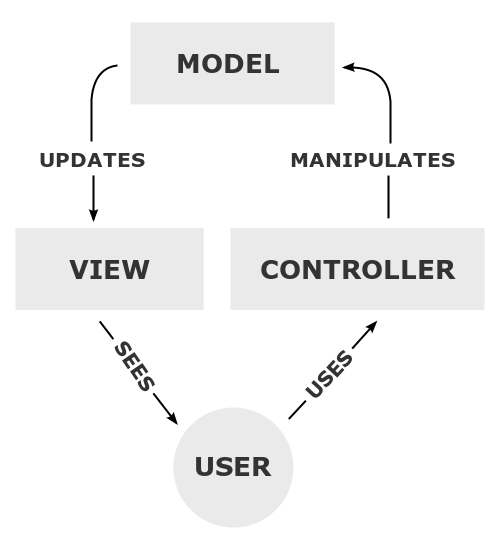
\includegraphics[height=9cm]{MVC-Process.png}
\subsection{View Interface}
\subsubsection{FXApp}
\subsubsection{FXController}
\subsubsection{DiningTableRow}
\subsection{Model Interface}
\subsection{Controller Interface}
\section{Dynamic Models of System Interface}
\subsection{Add Food Item Scenario}
\subsection{Remove Food Item Scenario}
\subsection{Set Food Item as Consumed Scenario}
\subsection{Set Food Item as Unconsumed Scenario}
\subsection{Hide Consumed Diet Scenario}
\subsection{Unhide Consumed Diet Scenario}
% add other chapters and sections to suit
\end{document}
